\chapter{Persistent Memory: Writing, Consolidation, Validity, and Influence}\label{ch:C14}

RecMem consolidates through recurrence-sensitive write stages, whereas October's Hy-Memory learns a memory writer from attributed feedback~\cite{dai2026recmem,fei2026hymemory}. InMind shows why stored or directly recallable information must still be tested for appropriate indirect influence~\cite{inmind2026}. The comparison unit is consequently the complete write--represent--retrieve--use lifecycle, including validity, delayed feedback, and the cost of maintenance.

\section{Memory functions and physical substrates}\label{sec:C14:taxonomy}
Agent memory is a collection of mechanisms for preserving, transforming, locating, and applying information across decisions. Working memory describes the task-relevant information currently available for control. Episodic memory preserves contextualized experience, including what was attempted, observed, and concluded in a particular situation. Semantic memory represents more reusable propositions or abstractions. These are functional distinctions. A vector database can store episodes or semantic statements, and one text document can contain both. The storage technology does not determine the memory function.

Biological terminology can motivate questions about consolidation, salience, interference, and forgetting, but it does not establish a shared implementation. A transformer context is not a demonstrated model of human working memory, and a graph of extracted facts is not a biological semantic system. Parametric knowledge, key-value caches, external records, and application state have different update and access mechanisms. The memory surveys provide useful taxonomies of forms, functions, and dynamics while also revealing how heterogeneous the underlying mechanisms are~\cite{corpus251213564,corpus260206052}.

Represent a memory object as
\begin{equation}
 m=(x,k,p,\tau_v,\tau_o,\sigma,\omega,v),
\end{equation}
where $x$ is content, $k$ its functional type, $p$ provenance, $\tau_v$ valid time, $\tau_o$ observation time, $\sigma$ confidence or status, $\omega$ ownership and access scope, and $v$ its version. This schema is proposed synthesis. It is deliberately richer than an embedding and text pair because future decisions can depend on whether a record is a direct observation, a tentative inference, or an obsolete preference. Embedding proximity alone does not supply those distinctions.

Working context should contain selected memory objects and the metadata needed to interpret them. A persistent store can retain a much larger set, but persistence does not ensure that the right item is retrieved or used. A useful evaluation separates admission, retention, retrieval, interpretation, and action. A failure at the final action can originate in any earlier stage. Treating all failures as ``forgetting'' obscures whether the information was absent, inaccessible, misclassified, or correctly retrieved but improperly applied.

Three changes should also remain separate: adding an external record, updating a reusable procedure, and changing model parameters. All can alter future behavior, but only the third changes the parameterized policy directly. A memory method around a frozen model can improve task outcomes without demonstrating continual weight learning. This distinction becomes important when a product or paper uses ``learning'' to describe a growing external store. The mechanism should be identified before its generality or long-term stability is assessed.


% SCIENTIFIC_FIGURE_C14
Figure~\ref{fig:C14:overview} shows the distinct curation and selection operations between history, typed stores, and working context.
\begin{figure}[!htbp]
\centering
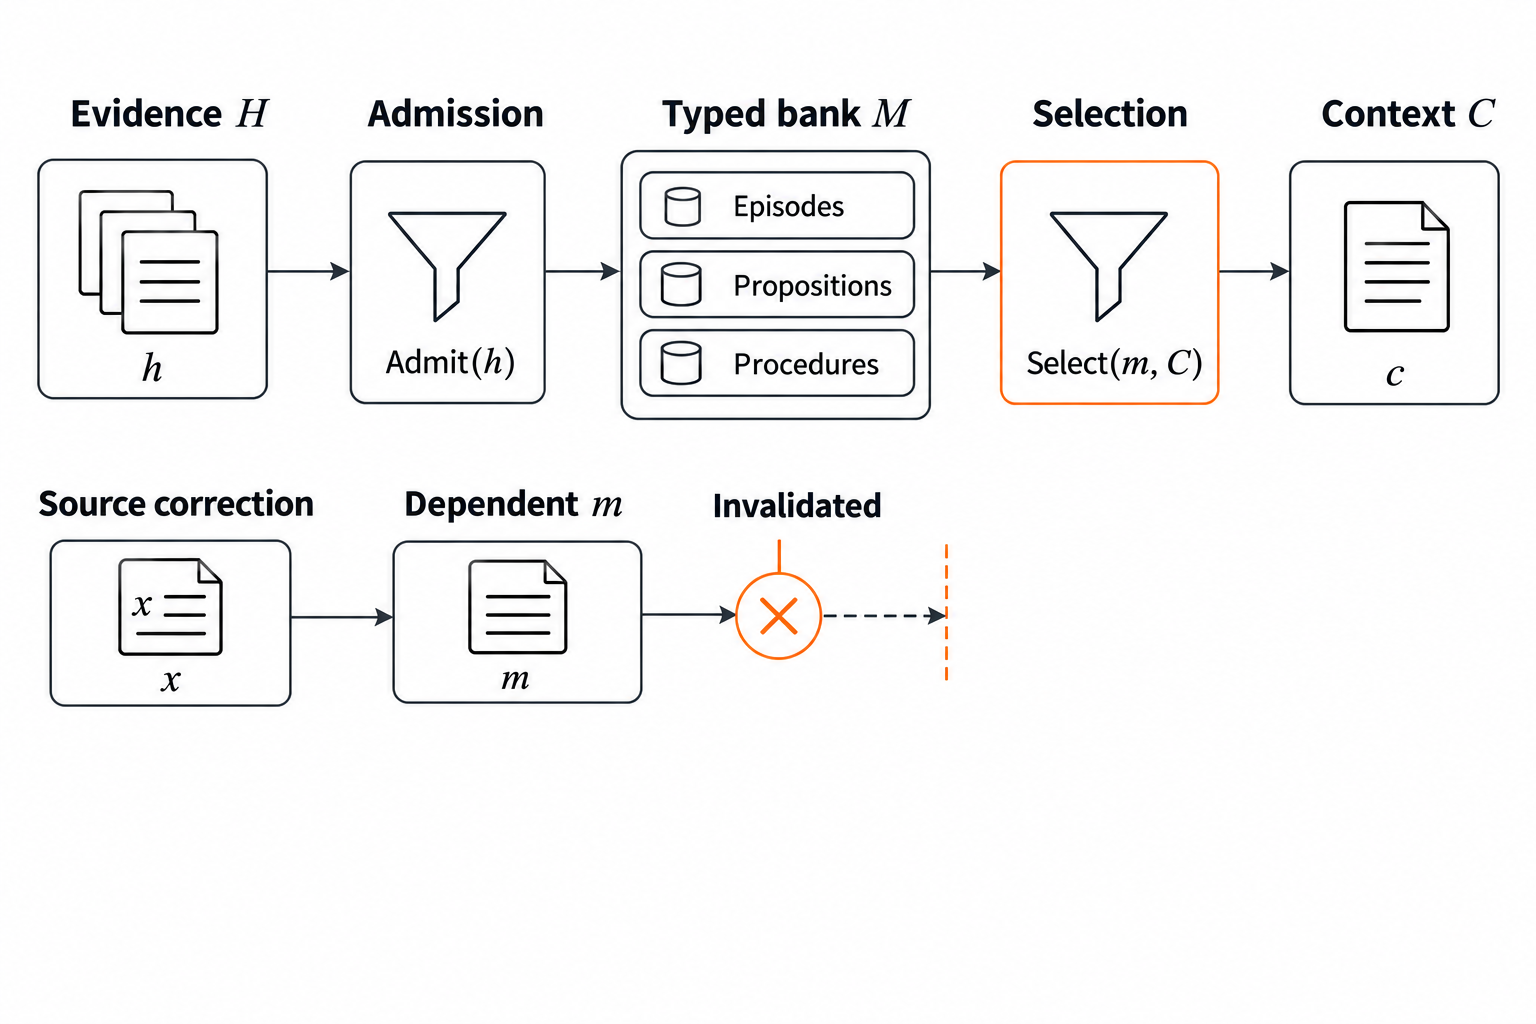
\includegraphics[width=\linewidth]{book/figures/assets/F14review.png}
\caption{Typed retention and invalidation. Evidence $h$ from history $H$ is admitted into a bank $M$ of episodic, propositional and procedural objects. Selection supplies working context $c$; an invalidated dependent object $m$ is blocked pending its specified revalidation. Publication status and provenance remain part of each object record. Current authorization is a separate boundary omitted here. Arrows show lifecycle dependencies, not guaranteed truth or universal conversion between classes. Here $C$ names the working-context component and $c$ its constructed content.}
\label{fig:C14:overview}
\end{figure}

\section{Admission as a constrained decision}\label{sec:C14:admission}
Writing every observation is inexpensive only when storage, indexing, privacy, and later interference are ignored. Generated tool output can contain duplicate text, stale state, adversarial instructions, and transient failures. Admission decides which records enter a persistent store, at what level of abstraction, and with what provenance. It should distinguish retaining raw evidence for audit from promoting a proposition into reusable semantic memory.

Let $\mathcal L(M)$ be expected future decision loss when the evaluated reader and retrieval policy use bank $M$. Define its decision value as $U(M)=\mathcal L(\varnothing)-\mathcal L(M)$. With $c_s(m)$ denoting storage and maintenance cost, $c_p(m)$ privacy or policy cost, and $r(m)$ estimated harmful-reuse risk, a proposed admission objective is
\begin{align}
 &\max_M\left\{U(M)-\sum_{m\in M}c_\lambda(m)\right\},\\
 &c_\lambda(m)=\lambda_s c_s(m)+\lambda_p c_p(m)+\lambda_r r(m),
\end{align}
subject to access and retention constraints. The nonnegative weights put the penalty terms on the decision-loss scale; their additive form is an accounting approximation, not an assumption that decision value is additive. The value of admitting $m$ is conditional on the bank, $\Delta(m\mid M)=U(M\cup\{m\})-U(M)$. An identifier and its disambiguating scope can each be useless alone and decisive together. A stale instruction can instead make adding a record harmful. Neither monotonicity nor diminishing returns follows from the memory label. These quantities depend on future tasks and the consumer policy, so the objective specifies an estimand rather than a solved scorer. A one-time authority correction should remain a control constraint even when a learned utility estimate is low.

Recurrence is one practical proxy for consolidation value. RecMem buffers interactions with embeddings and triggers more expensive episodic and semantic extraction around recurring related content~\cite{dai2026recmem}. Its semantic refinement revisits associated raw interactions to recover details omitted by an episodic abstraction. This trades eager extraction for a recurrence-conditioned pipeline. The paper evaluates conversational-memory tasks, not indefinite autonomous execution. Its heuristic thresholds and the possibility of rare but important information limit generalization from average recall results.

The inspected implementation makes the gate concrete. In the \texttt{RecMem} class, \path{add_memory} first attempts an episodic merge. Otherwise it searches raw-memory neighbors, filters by a similarity threshold, and compares the resulting count plus the incoming item with a consolidation count. The non-triggered path inserts the raw message with a timestamp; the triggered path calls \path{_consolidate_memory}~\cite{repo_recmem2026}. Thus the decision depends on both existing episodic coverage and raw recurrence. Describing it only as ``three-layer memory'' would omit the mechanism that determines its construction cost.

A deployment should add a separate pinning rule for information whose consequence is not well estimated by frequency. This is a design deduction, not a reported feature or result of RecMem. Examples include current authority, explicit user prohibitions, identifiers needed for reconciliation, and unresolved safety constraints. Such objects can remain in typed state even when ordinary conversational content follows recurrence-based consolidation. The resulting hybrid admits that one salience heuristic need not govern every memory class.

Personalized admission has a further feedback asymmetry. The October 2026 gating study formulates storage decisions with delayed, one-sided feedback: subsequent use can label an admitted fact, whereas the corresponding evidence for a discarded fact is unavailable. Its Warm-Start UCB method transfers a prior from other profiles and adapts through confidence-based exploration; the analysis assumes a specified linear utility model and a sufficiently accurate prior region~\cite{ji2026gating}. Neither a missing retrieval hit nor a currently pending label proves uselessness. Moreover, retrieval-confirmed use is a proxy for utility, not an independent measurement of improved user outcomes. Logging the label deadline, retrieval policy, and admission propensity is necessary to distinguish feedback delay from selection bias and from genuine preference change.

The reported LoCoMo comparison with GPT-4.1-mini is instructive because the full-context reference remains stronger in accuracy while requiring no memory-construction stage. Table~\ref{tab:C14:recmem} separates accuracy from construction tokens; the latter exclude the complete query-time and infrastructure boundary. The values are author-reported and not independently reproduced.
\begin{table}[htbp]\centering\small
\caption{RecMem's reported LoCoMo configuration~\cite{dai2026recmem}. Construction tokens are in thousands.}\label{tab:C14:recmem}
\begin{tabular}{L{36mm}rr}\toprule
Method & Accuracy (\%) & Construction tokens\\\midrule
Full context & 84.18 & 0.00\\
Mem0 & 62.92 & 1520.80\\
RecMem & 81.10 & 193.20\\\bottomrule
\end{tabular}
\end{table}


\section{Episodic records and abstraction loss}\label{sec:C14:episodes}
An episode should preserve the relationship between the situation, the policy's attempt, the observation, and the evaluated outcome. A useful record distinguishes a successful action from a plausible explanation of why it succeeded. If the environment returned a success signal, the agent can record that signal. Inferring a general strategy from the signal is a further abstraction. Keeping those layers separate prevents one lucky trajectory from becoming an apparently validated rule.

Let a trajectory be $\xi=(o_0,a_0,o_1,\ldots,a_{T-1},o_T)$ and let $z=s(\xi)$ be its episodic abstraction. A downstream retrieval query may need an exact error message, a resource identifier, or a failed alternative that the summary omitted. The abstraction's quality depends on the future query distribution, as in Chapter~\ref{ch:C11}. A narrative that captures the overall task can still be insufficient for a later repair. Store a pointer to the source trajectory when retention permits, and preserve exact evidence fields that support verification.

RecMem's code illustrates a nontrivial failure boundary. Its consolidation routine sorts existing raw neighbors by timestamp and then appends the incoming record, rather than inserting it into that chronological order. It constructs episodic memories and proceeds to semantic refinement. If episodic generation returns no records, it returns before deleting raw neighbors. If semantic extraction returns no facts, the inspected path can still proceed to remove consolidated raw items~\cite{repo_recmem2026}. These are implementation observations at the cited revision, not measured paper failures. A backdated incoming record provides a discriminating test of prompt order versus valid time; generation failure provides a separate test of which evidence survives each storage-layer transition.

There is a narrower ingestion gap on that early-return path: the incoming record is passed directly to consolidation, and the caller does not then insert it into the raw store. Preserving existing neighbors therefore does not prove that the newly arrived interaction remains recoverable. This is visible in the inspected control flow, not an independently reproduced loss event. A fault-injection test must check the incoming item separately from the old raw neighbors, with an upstream acknowledged event log as a distinct baseline.

The corresponding engineering question is atomicity of abstraction. Should raw evidence be removed only after every intended derivative is committed, or is the episodic artifact sufficient to justify removal? There is no universal answer. If the task requires fine-grained facts that episodic extraction can omit, deletion after partial refinement may reduce recoverability. If raw content has a strict retention limit, preserving it indefinitely can violate the application contract. The correct behavior requires an explicit transaction and retention policy.

Episode merging also risks losing exception structure. Two similar successes can differ in a precondition that later determines whether a procedure applies. Merging them into a generic account may hide that condition. An episode store should therefore preserve source membership and avoid claiming that a merged summary contains every distinction from its constituents. A proposed merge validator tests representative questions and action preconditions against both the originals and the candidate abstraction, with failures retained as counterexamples.

Outcome metadata needs comparable care. A task completed under oracle feedback, a permissive simulator, or an outdated tool version can be useful experience, but its outcome should not be treated as evidence for an unchanged production environment. The episode's environment and evaluator versions are part of its meaning. Without them, retrieval can faithfully surface experience whose apparent success rests on conditions that no longer hold.


\section{Semantic memory and the status of a proposition}\label{sec:C14:semantic}
Semantic memory attempts to represent reusable information without carrying the complete episode each time. Its advantage is efficient access to facts, preferences, and abstractions. Its risk is detaching a proposition from the conditions under which it was observed or inferred. A statement such as ``the service accepts this argument'' is incomplete without a service version, scope, and time. A preference such as ``use the fast route'' may apply to one task and not to every future decision.

Separate factual assertions, user preferences, procedures, hypotheses, and authority. They have different update rules. A new authoritative correction can supersede a preference; conflicting observations may require uncertainty rather than replacement; an explicit prohibition cannot be overridden by repeated assistant-generated statements. A semantic store that deduplicates solely by embedding similarity can merge records whose surface meanings overlap while their roles differ. Deduplication should preserve distinctions needed for future interpretation.

A proposed semantic update represents competing propositions as a set with status rather than forcing immediate collapse to one string. For entity $x$, predicate $p$, and value $y$, retain the source, valid interval, and confidence of each assertion. A resolver produces a current view according to explicit rules. For example, source authority can precede recency, and recency can be evaluated within the correct valid-time interval. This is a semantic policy, not merely a database ordering operation.

Generative Agents and MemGPT show different ways of organizing external information and making selected state available to an underlying model~\cite{park2023generativeagents,packer2023memgpt}. Their architectures motivate the separation between stored experience and active context. They do not establish that extracted statements are universally correct, that biological memory mechanisms have been reproduced, or that an agent can retain all important information indefinitely. Those are stronger claims requiring different evidence.

Semantic extraction can also amplify certainty. A source says that a method ``may help'' under a particular setting; a first summary says it ``helps''; a later consolidated memory says it is the preferred method. Each individual rewrite can look reasonable while the chain removes uncertainty and scope. Provenance should therefore be attached to assertions, and the system should preserve the original qualification where it affects decisions. Repeated generation is not independent corroboration.

An evaluation can construct paired records differing only in modality, scope, or authority: an observation versus a hypothesis, a project preference versus a global preference, and a user correction versus a retrieved recommendation. The memory system should preserve the distinction through extraction, merging, retrieval, and use. This proposed test directly measures whether semantic normalization erases operational meaning. Exact-match fact recall alone does not expose these role errors.


\section{Hierarchy access and complete lifecycle cost}\label{sec:C14:hierarchy}
A hierarchy can keep a small active state, a medium-sized abstraction layer, and a large evidence store. The hierarchy is useful when access frequencies and representation costs differ, but it introduces promotion, eviction, and synchronization policies. If a fact changes, every accessible derivative may need invalidation. If a summary is promoted to active state, it can displace another record whose future value was underestimated. The store layout and the control policy should be analyzed together.

Let $N_r,N_e,N_s$ be the numbers of raw, episodic, and semantic records. A naive dense retrieval over all embeddings has arithmetic cost proportional to $(N_r+N_e+N_s)d$ for embedding dimension $d$, before ranking and model generation. Approximate indexes change the cost-quality tradeoff and add index-maintenance work. A graph hierarchy can reduce some searches while increasing construction and traversal overhead. No storage representation is automatically more efficient without a specified query distribution and update rate.

RecMem's \path{search_memories} exposes three retrieval branches with separately configured limits and thresholds, returning raw, episodic, and semantic results~\cite{repo_recmem2026}. This matters for causal comparison: better answering can arise from more total evidence, different representation, or a different allocation across layers. A baseline that receives fewer retrieved tokens is not a clean test of consolidation structure. Match the complete evidence budget, and separately ablate which layer provides the decisive item.

Construction cost can dominate when many memories are written but few queries arrive. Query-time cost can dominate when a stable store serves many decisions. Let $C_w$ be total writing and consolidation cost, $C_q$ average retrieval-and-generation cost, and $Q\in\mathbb N_{>0}$ the number of useful queries. A simple amortized cost is $(C_w+QC_q)/Q$; it is undefined at $Q=0$, when construction produced no served query. This arithmetic explains why reporting only retrieval tokens can reverse the practical ranking of memory designs. Storage, indexing, failed extractions, and maintenance should remain inside the chosen boundary.

Cache and semantic invalidation also differ. Evicting a vector-search cache can cause recomputation without changing knowledge. Invalidating a false semantic proposition changes what future decisions should use. A hierarchical system must not use the same ``eviction'' operation for both without preserving the semantic reason. The working view should be able to tell whether an item is unavailable temporarily, deleted by retention, superseded by correction, or rejected as untrusted.

The practical implementation should record lifecycle counters by operation: admitted raw records, attempted extractions, successful episodes, semantic revisions, retrieval candidates, final injected items, invalidations, and deletions. These counters are diagnostic observables, not substitutes for task outcomes. They make it possible to explain why a method's cost or reliability changes with the number of sessions rather than reporting a single benchmark aggregate.

Hy-Memory-30B-A3B, introduced in an October 2026 technical report, instead targets a reusable writer inside several existing memory frameworks. It separates writer learning from the fixed reader used for reward, trains on policy-produced bank states, and combines per-chunk probes, attributed cross-chunk feedback, and a bank-growth penalty~\cite{fei2026hymemory}. Its reported cross-harness comparison uses fixed 20\% benchmark subsamples, including a held-out framework. That is evidence about a writer-reader-harness configuration, not a universal ranking of complete memory products. Its learned write protocol also differs from RecMem's training-free recurrence gate.

The comparison identifies a useful causal axis. RecMem changes when expensive abstraction is performed; Hy-Memory changes the policy performing framework-specific writes; HyperSkill changes the representation and maintenance of procedural experience. A result can improve because of any of these interventions, and combining their names does not establish a compatible composite system. A matched study would hold the reader and retrieval configuration fixed while varying admission timing, writer policy, and representation separately, then test interactions. In particular, a writer trained against one retriever can learn representations whose value disappears when the retrieval interface changes.


\section{Temporal validity conflicts and forgetting}\label{sec:C14:validity}
Prospective memory requires more than answering a question about the past: a future event must activate a previously established constraint. TriggerBench separates an early constraint from a later trigger using intervening dialogue, matched retrospective questions, overloaded positive triggers, and negative controls~\cite{zhang2026triggerbench}. Its distinction motivates an implementation object $(g,u,b)$: $g$ is a trigger predicate over observed events, $u$ is the intended intervention, and $b$ is an applicability boundary including expiry and authority. At an event, evaluate the guard and current boundary before proposing the intervention. This is a proposed representation, not a claim that the benchmark implements an event engine. Evaluate missed triggers and false activations separately; unconditional reminders can improve recall while failing negative cases. A reminder also cannot confer authority to execute the underlying action.

Memory usefulness depends on whether an assertion remains valid when it is used. A correct historical fact can be a wrong current instruction. A past failed attempt can be useful as an episode while its error cause has been fixed. Temporal validity should therefore be represented at the proposition or procedure level, not inferred from how recently a record was retrieved. Retrieval frequency measures access, not truth.

Use valid-time intervals $[t_b,t_e)$ where meaningful, and preserve observation time separately. If a user states at time $t_2$ that a preference changed at $t_1<t_2$, the current resolver should incorporate the earlier effective change without pretending the agent knew it before $t_2$. This supports both present decisions and historical audit. A last-write-wins store ordered by ingestion can produce the wrong historical answer, while a store ordered only by effective time can lose what was actually known at a decision.

Conflicts can be factual, temporal, procedural, or authoritative. Factual conflict concerns incompatible descriptions of the same state. Temporal conflict can disappear once intervals are distinguished. Procedural conflict concerns strategies with different preconditions. Authority conflict concerns who may direct an action. A generic contradiction prompt can help identify conflicts, but the resolver's rule must reflect the class. Majority voting over repeated model-generated statements is especially weak evidence of authority or truth.

Forgetting has several meanings: preventing retrieval, removing a record, deleting derivatives, expiring an active preference, or modifying parameters. An external memory system should state which operation it implements. Removing a row from one index does not establish erasure from raw logs, summaries, backups, or downstream services. Conversely, revoking future use can be a meaningful operational guarantee even when some audit record remains. Claims should follow the actual deletion and retention contract.

A proposed invalidation protocol marks the source assertion obsolete, finds derived summaries and skills that depend on it, invalidates their reusable status, and rebuilds any current view that included them. This assumes a recorded dependency graph. Missing provenance limits completeness. A safe fallback can quarantine a larger region of memory at the cost of reduced utility. That tradeoff should be measured rather than hidden behind a claim of perfect forgetting.

Longitudinal evaluation should include corrected facts, changed preferences, expired permissions, and requests to forget. Score not only the desired new answer but also whether the agent stops using the old record in unrelated later tasks. Include negative controls where an update should not affect another project or user. These tests assess selective revision rather than indiscriminate amnesia. Their relevance increases as sessions, teams, and model versions share a growing store.


\section{Retrieval does not imply appropriate use}\label{sec:C14:use}
Memory can fail through excessive influence as well as omission. MemSyco-Bench constructs decisions where relevant historical material must be rejected as factual evidence, bounded to its original scope, reconciled with current evidence, updated, or used for legitimate personalization~\cite{cumb2026memsycov3}. These categories distinguish retrieval success from epistemically appropriate use. A stored preference is evidence about a user's preference; it does not become evidence that the preferred claim is objectively correct. A discriminating counterfactual preserves the current evidence and changes only the historical preference. An objective answer should remain invariant, while a preference-dependent recommendation may appropriately change. That conditional distinction is stronger than rewarding either universal obedience to memory or universal suppression.

Response concentration is a separate outcome. The October MemBubble benchmark derives preferences from real conversations and constructs topically related queries in distinct scenarios, then measures diversity using functional-equivalence classes of sampled answers~\cite{tan2026membubble}. Its query filtering and diversity pre-test define a selected evaluation population; the result cannot estimate all deployment queries without a sampling argument. An original evaluation recommendation is to report valid-personalization accuracy and response-distribution concentration jointly. Higher entropy can include irrelevant alternatives, while lower entropy can reflect a justified constraint. Hold the decoder and sampling budget fixed, inspect the equivalence-class judge, and separate memory-induced narrowing from changes already implied by the current request.

An agent can store a fact, retrieve it when asked directly, and fail to apply it when relevance is implicit. InMind isolates this distinction with paired storage and in-context controls and an answer-blind target-recall measurement~\cite{inmind2026}. Its 125-task diagnostic reports a large gap between direct recall and application under indirect queries. The result concerns the tested systems and selected implicit associations, not every possible retrieval mechanism. Missing broad negative controls also matters when evaluating whether a remedy overapplies memory.

The mechanism is a sequencing problem. A query-conditioned retriever must decide what is relevant before the full policy sees the candidate fact. If relevance depends on a bridge supplied by world knowledge, surface similarity can miss it. Increasing embedding dimensionality does not necessarily solve the need to infer that bridge. A structured profile, proactive constraint store, query expansion, or model-assisted memory search can change the access interface, but each introduces a different cost and failure mode.

The official InMind artifact makes the evaluation boundary inspectable. Its timeline builder constructs the ordered conversation for a selected task, while its judge-payload builder separates measurements through metric-specific payloads~\cite{repo_inmind2026}. These are benchmark construction and scoring paths rather than a released solution to the memory-use problem. A reproduction must preserve the paired controls, target-fact placement, answer-blind measurement, and system output schema. Omitting a control can turn a retrieval diagnosis into an ambiguous end-to-end failure.

InMind's reported in-context control reaches 84.0\%, while the six evaluated memory systems reach at most 14.4\% on indirect application and can reach 100\% on direct recall~\cite{inmind2026}. The separately evaluated dense NaiveRAG baseline reaches 16.0\% on indirect application; it is not included in that six-system maximum. These percentages have different experimental conditions and should not be subtracted as if they were a randomized treatment effect. The official timeline code also freezes the post-history state for direct and indirect queries, preventing one query's answer from teaching the subsequent query the target fact. This control is crucial: sequentially asking the direct question first would change the state and confound the diagnosis.

Appropriate use also requires authority calibration after retrieval. A memory can be relevant as background evidence without being a binding constraint. A tentative preference should not override a current explicit instruction, and an old successful procedure should not override a changed tool contract. One proposed interface labels each item with its role: observation, preference, candidate procedure, or current obligation. The model still interprets the item, while deterministic controls can prevent some role promotions at consequential boundaries.

Formally, let $z$ denote the current task state and $m$ a retrieved item. The useful question is the change in expected loss caused by making $m$ visible, conditional on its status and provenance. Similarity is a retrieval signal; causal usefulness is an outcome under an intervention. Estimating the latter requires matched continuations or randomized memory exposure where appropriate. Observational correlation between retrieval and success is confounded because easier or familiar tasks can both retrieve better and succeed more often.

An evaluation should include four conditions: the fact absent, present in storage, explicitly retrieved, and permanently visible as a diagnostic control. Compare action correctness and inappropriate-use rates, not only answer recall. If explicit exposure repairs performance, the bottleneck is likely upstream of use under those conditions. If it does not, missing bridge knowledge or interpretation remains possible. This decomposition gives a concrete experimental route from an aggregate memory score to a mechanism-specific conclusion.

\subsection{Identifying memory influence}
A controlled exposure study can make the causal estimand explicit. Let $X_i$ bind a frozen task, memory-bank snapshot and model configuration. Let $B_i\in\{0,1\}$ indicate whether one eligible memory item is exposed, with known assignment probability $e_i=P(B_i=1\mid X_i)\in(0,1)$. Write $L_i(1)$ and $L_i(0)$ for the two potential decision losses and observe $L_i=B_iL_i(1)+(1-B_i)L_i(0)$. Under randomized assignment conditional on $X_i$, consistent exposure, and no cross-trial state interference,
\begin{equation}
 \widehat\Delta_n=\frac1n\sum_{i=1}^n
 \left[\frac{B_iL_i}{e_i}-\frac{(1-B_i)L_i}{1-e_i}\right]
\end{equation}
has expectation $n^{-1}\sum_i\mathbb E[L_i(1)-L_i(0)]$, the average exposure effect for the sampled task population. The identity follows by conditioning each term on $X_i$ and its potential losses. Negative $\Delta$ means beneficial exposure on this evaluated distribution. Very small propensities can make the estimator unstable, so uncertainty and the assignment range must be reported.

This construction is a proposed experiment, not a measured memory benefit. Use sandboxed or read-only continuations with reset state where withholding evidence is permissible; current authorization and mandatory obligations are not randomized away. A shared persistent bank updated by earlier trials breaks the no-interference premise unless the trajectory itself is the randomized unit. Delayed or missing labels require an additional observation model: logging admission propensity alone does not identify outcomes for permanently censored facts. The experiment also distinguishes the influence of an item from its factual correctness and from the quality of the writer that produced it.

\section{Memory transactions and a reference test suite}\label{sec:C14:transactions}
Memory construction often spans several writes: raw evidence, embeddings, an episode, semantic propositions, and provenance links. A partial failure can leave these layers inconsistent. The central transaction question is which combinations constitute a valid published memory state. If the semantic record references an episode that never committed, retrieval can return an unsupported assertion. If the raw item is removed before the episode becomes durable, recovery can lose both evidence and abstraction.

A proposed two-stage publication process first writes candidate derivatives with explicit source references and pending status. Validation checks schemas, provenance existence, ownership, and any required exact fields. A commit then makes the derivatives retrievable and records whether raw evidence may be removed under retention rules. Failed candidates remain unavailable to the answer policy. This is an implementation pattern, not an established universal memory algorithm. Semantic validity still requires stronger checks than database atomicity.

For a conservative publication gate, let $D(m)$ be the recorded transitive dependencies of candidate $m$, $c(m)$ its committed-status bit, and $a_{\alpha,t}(m)$ its current access-and-validity check. A strictly source-bound view can expose
\begin{equation}
 M_{\alpha,t}^{\rm vis}=
 \{m:c(m)=1,\ a_{\alpha,t}(m)=1,
        \ a_{\alpha,t}(x)=1\ \forall x\in D(m)\}.
\end{equation}
This is a proposed policy, not a necessary rule for every legitimate aggregate. It assumes complete dependency recording and current checks; missing lineage requires unresolved status or a broader quarantine. It certifies publication structure and scope, not the semantic truth of $m$. A correction can revoke reusable status without falsifying the historical event that an old version was used. Effect receipts and current grants therefore retain their typed control semantics instead of becoming ordinary similarity-ranked facts.

The state can maintain separate read and write versions so that an ongoing task sees a coherent memory snapshot. A new correction can trigger explicit refresh rather than silently changing the evidence beneath a multi-step plan. For high-consequence obligations, refresh may need to occur immediately before tool execution. For ordinary background facts, snapshot consistency may be adequate. The choice follows workload consequences and should be specified per memory class.

The proposed test suite includes extraction failures, duplicate writes, interrupted consolidation, stale embeddings after a correction, conflicting user scopes, and a summary whose source has expired. Each case has a deterministic structural oracle where possible and a separately evaluated semantic outcome. Compare a raw-log baseline, a flat fact store, a layered store, and a structured obligation profile under the same backbone and complete cost boundary. Report task order and repeat runs because the store evolves during evaluation.

For RecMem-like recurrence policies, vary the frequency of decisive facts independently of their importance. This tests whether recurrence is a useful cost proxy without making frequency and utility identical by benchmark construction. For semantic merging, create near-duplicate records with different temporal scope or authority. For retrieval-use failures, retain the InMind-style paired controls. For deletion, test derived artifacts and cross-session behavior rather than only a missing database row. These are proposed experiments, not new results.

The resulting engineering standard is precise but bounded. A memory system should say what it stores, when it consolidates, how it retrieves, which authority its records carry, how it handles corrections, and what its transaction protects. It should not claim lifelong continuity from successful direct recall, or parametric learning from external storage growth. Procedural consolidation in Chapter~\ref{ch:C15} extends this analysis to reusable skills whose errors can influence many later tasks.

